\chapter{Cơ sở lý thuyết}
Chương này sẽ giải thích về chuỗi thời gian và chuỗi con bất thường ở mục 2.1 và 2.2, tiếp theo trình bày chi tiết về lý thuyết về các kiến trúc mạng nơ-ron được chúng tôi áp dụng để nghiên cứu, cũng như cách xây dựng mô hình mạng nơ-ron học sâu LSTM xếp chồng trong các mục 2.3, 2.4, 2.5 và 2.6. Các cơ sở lý thuyết này sẽ được sử dụng để xây dựng một mạng nơ-ron học sâu LSTM xếp chồng nhằm mục đích dự báo dữ liệu chuỗi thời gian và phát hiện bất thường.

\section{Chuỗi thời gian và dự báo chuỗi thời gian}
\textit{Chuỗi thời gian (Time Series):} Chuỗi thời gian \textit{T} = $t_1$,...,$t_m$ là tập hợp \textit{m} các giá trị thực được đo đạc tại những điểm thời gian cách đều nhau.

Hình \ref{fig:2-1} minh họa một chuỗi thời gian theo dõi quá trình đo nhiệt độ tại một địa phương

\begin{figure}[H]
    \centering
    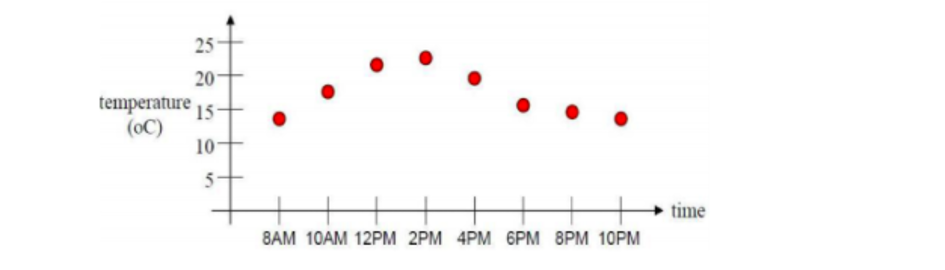
\includegraphics[scale=0.95]{./content/images/2-1.png}
    \caption{Chuỗi thời gian}
    \label{fig:2-1}
\end{figure}

Trong thực tế, có rất nhiều loại dữ liệu chuỗi thời gian như sự theo dõi biến động giá chứng khoán, dữ liệu điện tâm đồ, dữ liệu theo dõi sự truy cập các trang web của người dùng,... Thông thường, các loại dữ liệu chuỗi thời gian này là rất lớn, được đo và lưu trữ lại trong một khoảng thời gian dài cho nên việc khai phá dữ liệu này thường tốn kém chi phí thời gian. Do đó việc sử dụng các công cụ khai phá dữ liệu này được áp dụng trên nền máy tính đã thu hút sự quan tâm, nghiên cứu và ứng dụng trong rất nhiều các lĩnh vực trong những năm gần đây.


Một số vấn đề có thể xảy ra khi khai phá dữ liệu chuỗi thời gian:
\begin{itemize}
    \item  \textbf{Khối lượng dữ liệu}: Một trong những đặc trưng của chuỗi thời gian là dữ liệu rất lớn. Đây là một trong những vấn đề thách thức trong quá trình phân tích, tính toán và xử lý dữ liệu chuỗi thời gian trong việc tạo ra kết quả được chính xác trong thời gian hợp lý?
    \item \textbf{Phụ thuộc yếu tố chủ quan}: Trong thực tế, các kết quả dữ liệu chuỗi thời gian thu được chịu ảnh hưởng yếu tố chủ quan của người đo dữ liệu, điều kiện và các công cụ đo…
    \item \textbf{Dữ liệu không đồng nhất}: Quá trình thu thập dữ liệu chuỗi thời gian được đo trên những định dạng khác nhau, số lượng và tần số lấy mẫu không đồng nhất cũng ảnh hưởng đến tính toàn vẹn của dữ liệu. Thêm vào đó quá trình đo đạc không chính xác do nhiễu, thiếu một vài giá trị hay dữ liệu không sạch.
\end{itemize}

Dữ liệu chuỗi thời gian được phân ra thành 2 nhóm chính:
\begin{itemize}
\item \textbf{Chuỗi thời gian đơn biến}: như tên gọi của nó, là một chuỗi có một biến phụ thuộc thời gian duy nhất. Ví dụ như: năng lượng tiêu thụ trong một tuần, giá trị điện tâm đồ,... 
\item \textbf{Chuỗi thời gian đa biến}: chuỗi thời gian có nhiều hơn một biến phụ thuộc vào thời gian. Mỗi biến không chỉ phụ thuộc vào các giá trị trong quá khứ của nó mà còn có một số phụ thuộc vào các biến khác. Sự phụ thuộc này được sử dụng để dự báo các giá trị trong tương lai. Ví dụ như: giá trị cỗ phiếu từng ngày trong một tuần,..
\end{itemize}

\section{Chuỗi con và chuỗi con bất thường}
\subsection{Chuỗi con}
\textit{Chuỗi con (Subsequence)}: Cho một chuỗi thời gian \textit{T} có độ dài \textit{m}, một chuỗi con \textit{C} của \textit{T} là một mẫu (sample) có độ dài \textit{n} $\leq$ \textit{m} lấy từ \textit{T}, nghĩa là \textit{C} = $t_p$,...,$t_{p+n-1}$ với 1 $\leq$ \textit{p} $\leq$ \textit{m} - \textit{n} + 1.

\subsection{Chuỗi con bất thường}
Một mẫu bất thường trên dữ liệu chuỗi thời gian là một chuỗi con mà rất khác so với chuỗi con tương tự với nó nhất. Tuy nhiên, những chuỗi con mà khớp (tương tự) với một chuỗi con cho trước thường có khuynh hướng gần sát với vị trí của chuỗi con đang xét. Thí dụ, một chuỗi con có vị trí bắt đầu tại điểm thứ \textit{p} có chuỗi con tương tự với nó nhiều nhất bắt đầu tại điểm thứ \textit{q} mà \textit{q} chỉ cách xa \textit{p} khoảng vài điểm. Những sự trùng khớp với nhau như vậy được gọi là \textit{trùng khớp tầm thường} (trivial matches) và không đáng quan tâm trong quá trình phát hiện bất thường.

\textbf{Định nghĩa 1: (Trùng khớp không tầm thường)} Một chuỗi thời gian \textit{T} cho trước có chứa chuỗi con \textit{C} chiều dài \textit{n} bắt đầu tại vị trí \textit{p} và một chuỗi con \textit{M} trùng khớp với nó bắt đầu tại vị trí \textit{q}, ta bảo \textit{M} là \textit{trùng khớp không tầm thường} (non-trivial match) của \textit{C} nếu |\textit{p} – \textit{q}| $\geq$ \textit{n}.

\textbf{Định nghĩa 2: (Chuỗi con bất thường nhất – time series discord)} Cho chuỗi thời gian \textit{T}, chuỗi con \textit{C} có chiều dài \textit{n} bắt đầu tại vị trí \textit{p} được gọi là chuỗi con bất thường nhất của \textit{T} nếu \textit{C} có khoảng cách lớn nhất đến chuỗi con trùng khớp không tầm thường lân cận với nó nhất. 

Chúng ta cũng quan tâm đến việc xem xét các chuỗi con bất thường bậc \textit{K} mà được định nghĩa như sau:

\textbf{Định nghĩa 3: (Chuỗi con bất thường bậc \textit{K} – \textit{K-th} time series discord)}  Cho chuỗi thời gian \textit{T}, chuỗi con \textit{D} có chiều dài n bắt đầu tại vị trí \textit{p} được gọi là chuỗi con bất thường bậc \textit{K} của \textit{T} nếu \textit{D} có khoảng cách lớn thứ \textit{K} đến chuỗi con trùng khớp không tầm thường lân cận với nó nhất và không hề phủ lấp chuỗi con bất thường bậc \textit{i} nào bắt đầu tại vị trí $p_{i}$, với mọi \textit{i} thỏa 1 $\leq$ \textit{i} $\leq$ \textit{K}.

\section{Phương pháp xấp xỉ gộp từng đoạn}
Phương pháp \textit{xấp xỉ gộp từng đoạn} (Piecewise Aggregate Approximation - PAA) do Keogh và cộng sự đề nghị năm 2001(\cite{st35}). Phương pháp này rất đơn giản, ta tuần tự xấp xỉ \textit{k} giá trị liền kề nhau thành cùng một giá trị bằng trung bình cộng của \textit{k} điểm đó. Quá trình cứ tiếp tục như vây từ trái sang phải, hình \ref{fig:2-3pp}. Với phương pháp này, thời gian tính toán rất nhanh và cách biểu diễn của nó hỗ trợ nhiều độ đo khoảng cách.

\begin{figure}[H]
    \centering
    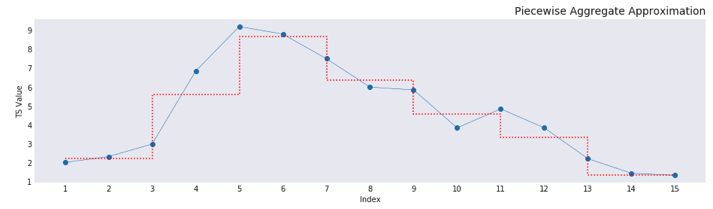
\includegraphics[scale=0.6]{./content/images/2-3pp.png}
    \caption{Phương pháp PAA}
    \label{fig:2-3pp}
\end{figure}

\section{Phương pháp xấp xỉ gộp ký hiệu hóa}
Lin và các cộng sự đã đề xuất phương pháp \textit{xấp xỉ gộp ký hiệu hóa} (Symbolic Aggregate approXimation - SAX) vào năm 2003 \cite{st36} để thực hiện rời rạc hóa dữ liệu chuỗi thời gian. Chuỗi thời gian ban đầu được chia thành từng đoạn bằng phương pháp PAA. Sau đó, dựa trên giá trị trung bình cộng của từng đoạn, ta sẽ biểu diễn đặc trưng của đoạn thành các ký tự. Khi đó, chuỗi thời gian ban đầu sẽ được mã hóa rời rạc thành một chuỗi các ký tự
như hình \ref{fig:2-3p}. Phương pháp này biểu diễn dữ liệu chuỗi thời gian thành dạng chuỗi ký tự nên từ đó có thể áp dụng được các kỹ thuật xử lý trên dữ liệu tràng ký tự để thực hiện xử lý, phân tích dữ liệu chuỗi thời gian.

\begin{figure}[H]
    \centering
    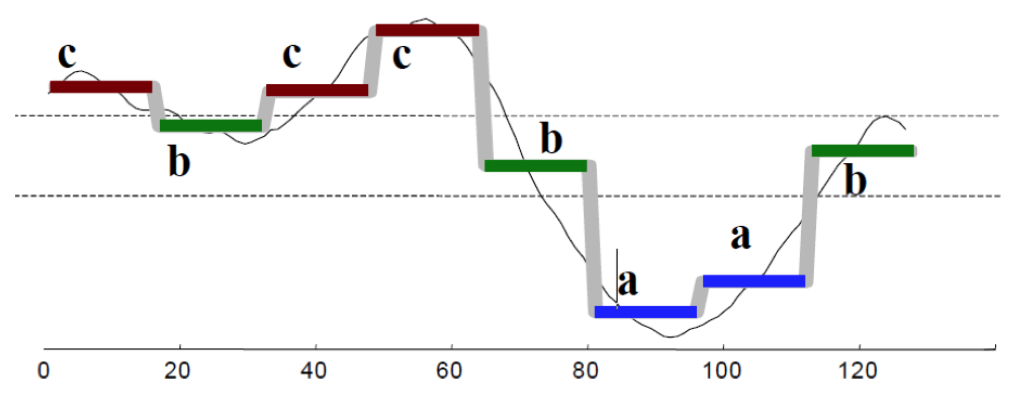
\includegraphics[scale=0.3]{./content/images/2-3p.png}
    \caption{Phương pháp SAX}
    \label{fig:2-3p}
\end{figure}

Phương pháp rời rạc hóa SAX giả định dữ liệu chuỗi thời gian phải thỏa phân phối Gauss và đã được chuẩn hóa bằng phép chuẩn hóa z-score. Khi đó, chúng ta có thể xác định các \textit{điểm ngắt} (breakpoint) để tạo ra các vùng có diện tích bằng nhau dưới đường cong phân phối Gauss. Số lượng điểm ngắt này tùy thuộc vào kích thước của \textit{tập ký tự} (alphabet) mà người dùng muốn sử dụng để ký hiệu hóa chuỗi thời gian. \textit{Kích thước} (size) của tập ký tự chính là thông số \textit{a} của phương pháp rời rạc hóa SAX. Thí dụ tập ký tự mà chúng ta muốn sử dụng là $\{$a, b, c, d$\}$ thì thông số \textit{a} được xác định là 4 và số điểm ngắt là 3.

\textbf{Định nghĩa:} \textit{Điểm ngắt} (breakpoint): Các điểm ngắt là danh sách các trị số có thứ tự \textit{B} = $\beta_{1},..., \beta_{a-1}$ sao cho diện tích dưới đường cong phân bố Gauss \textit{N}(0,1) từ $\beta_{i}$ đến $\beta_{i+1}$ bằng 1/\textit{a} (trong đó $\beta_{0}$ và $\beta_{a}$ lần lượt là $-\infty$ và $\infty$). Các điểm ngắt có thể được xác định theo kích thước tập ký tự \textit{a} nhờ vào hình \ref{fig:2-4p}

\begin{figure}[H]
    \centering
    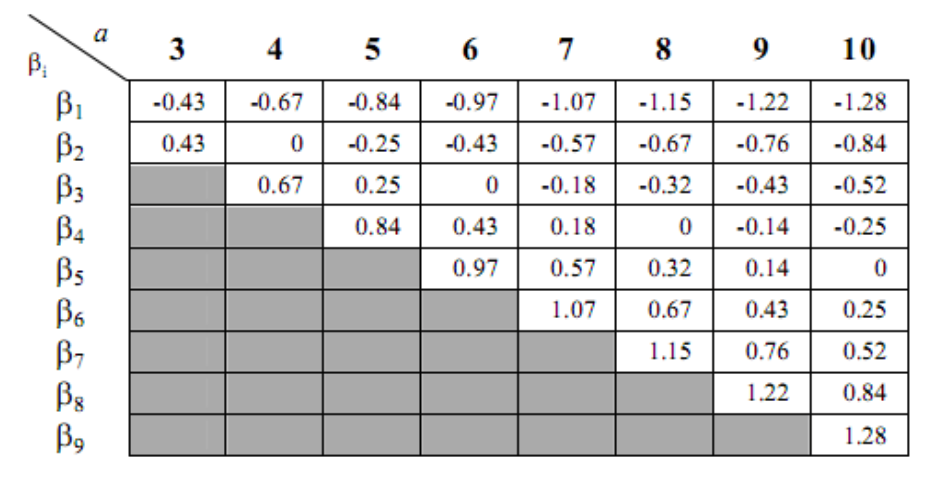
\includegraphics[scale=0.45]{./content/images/2-4p.png}
    \caption{Bảng tra tìm các giá trị $\beta$ theo từng giá trị \textit{a} tương ứng}
    \label{fig:2-4p}
\end{figure}

Khi đã xác định được tập các điểm ngắt, chuỗi thời gian sẽ được rời rạc hóa theo cách sau đây:
\begin{itemize}
\item Tất cả các giá trị PAA nhỏ hơn giá trị điểm ngắt nhỏ nhất ánh xạ thành ký tự “\textbf{a}”.
\item Tất cả giá trị PAA lớn hơn hoặc bằng giá trị điểm ngắt nhỏ nhất và nhỏ hơn giá trị điểm ngắt nhỏ thứ hai ánh xạ thành ký tự “\textbf{b}”, cứ tiếp tục như vậy cho đến hết chuỗi.
\end{itemize}

\section{Mạng nơ-ron nhân tạo (Artiticial Neural Networks - ANN)}
Qua quá trình nghiên cứu về bộ não, các nhà khoa học nhận thấy rằng: Hệ thần kinh con người được mô tả là một hệ thống gồm 3 phần tử chính bao gồm các \textit{đầu dây thần kinh cảm ứng} (receptors), \textit{hệ thống thần kinh trung tâm} (brain, neural nets) và \textit{hệ thống chấp hành} (effectors). Các thần kinh cảm ứng thu thập các tác động từ môi trường bên ngoài, chuyển thành tín hiệu điện và chuyển về hệ thần kinh trung ương. Tại đây, các tín hiệu sẽ được não bộ phân tích, xử lý và đưa ra các quyết định điều khiển. Các tín hiệu điều khiển này sẽ được chuyển tới các cơ quan chấp hành để thực hiện. Trong đó, nơ-ron là phần tử cơ bản của hệ thần kinh.

ANN là mô hình tính toán được xây dựng dựa trên ý tưởng của nơ-ron sinh học. Nó gồm các nơ-ron nhân tạo nối với nhau, và xử lý thông tin bằng cách truyền theo các kết nối và tính giái trị mới tại các nơ-ron. Về mặt lý thuyết, ta có thể xây dựng một mạng với cách kết nối tùy ý. Tuy nhiên phổ biến nhất là \textit{mạng truyến thẳng} (multilayer perception - MLP). Mạng MLP là một mạng truyền thẳng với các khối cơ bản là các nơ-ron McCulloch-Pitts. Ngoài ra mạng MLP còn có một số yêu cầu sau về cấu trúc của mạng:
\begin{itemize}
\item Các nơ-ron được sắp xếp thành các \textit{tầng} (layer), mạng gồm một tầng gồm các kênh tín hiệu đầu vào (input layer), một tầng gồm các kênh tín hiệu đầu ra (output layer) và có thể gồm một số tầng trung gian gọi chung là các tầng ẩn (hidden layer).
\item Không có các kết nối giữa các nơ-ron trên cùng một tầng mà chỉ có các kết nối giữa các nơ-ron của hai tầng liên tiếp. Các kết nối đều có chiều hướng đi từ đầu vào đến đầu ra (mạng truyền thẳng).
\item Các nơ-ron trên cùng một tầng sẽ có cùng \textit{hàm truyền} (transfer function).
\end{itemize}

Hình \ref{fig:2-2} và \ref{fig:2-3} mô tả hai mô hình của mạng MLP.

\begin{figure}[H]
    \centering
    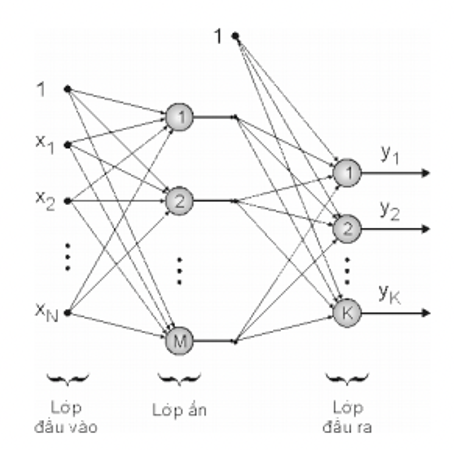
\includegraphics[scale=0.75]{./content/images/2-2.png}
    \caption{Mô hình mạng MLP với một tầng ẩn}
    \label{fig:2-2}
\end{figure}

\begin{figure}[H]
    \centering
    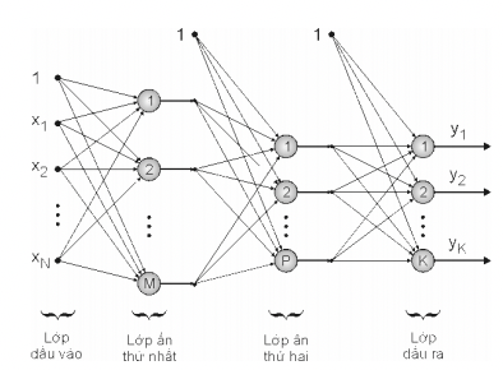
\includegraphics[scale=0.75]{./content/images/2-3.png}
    \caption{Mô hình mạng MLP với hai tầng ẩn}
    \label{fig:2-3}
\end{figure}

Về mặt lý thuyết, ta có thể xây dựng mạng MLP với số lượng tầng ẩn tùy ý, tuy nhiên các nghiên cứu đã chứng minh được rằng ta chỉ cần sử dụng tối đa hai tầng ẩn là có thể mô hình hóa một hàm phi tuyến với độ chính xác tùy chọn. Vì vậy trong thực tế ta thường chỉ các mạng không có hoặc có một hay hai tầng ẩn. Trong số đó phần lớn chỉ dùng mạng có một tầng ẩn do mạng không có tầng ẩn thì quá đơn giản, còn mạng có hai tầng ẩn trở nên lại quá phức tạp. Vì vậy trong các vấn đề được trình bày tiếp theo dưới đây sẽ sử dụng mạng có một tầng ẩn, các công thức cho mạng với cấu trúc khác có thể dễ dàng phát triển một cách tương tự.

Để thuận tiện cho việc theo dõi, trong các công thức của mạng MLP, ta có quy ước về đánh chỉ số các trọng số ghép nối giữa các phần tử của mạng như hình \ref{fig:2-4}: nếu phần tử ngọn có chỉ số là \textit{i} và phần tử gốc có phần tử là \textit{j} thì trọng số ghép nối giữa hai phần tử đó sẽ có chỉ số là \textit{ij}.

\begin{figure}[H]
    \centering
    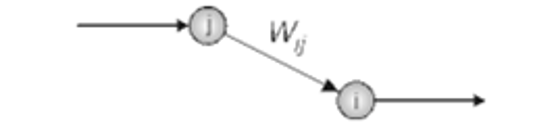
\includegraphics[scale=0.75]{./content/images/2-4.png}
    \caption{Quy ước đánh chỉ số các trọng số ghép nối giữa các nơ-ron}
    \label{fig:2-4}
\end{figure}

Cấu trúc một mạng MLP với một tầng ẩn, trong đó mạng có \textit{N} đầu vào, \textit{M} nơ-ron trên tầng ẩn và \textit{K} đầu ra. Như hình \ref{fig:2-5}, nếu ký hiệu chung các trọng số ghép nối giữa tầng đầu vào và tầng ẩn là $W_{ij}$ thì ta có \textit{i} = 1,2,...,\textit{M}; \textit{j} = 0,1,2,...,\textit{N}. Nếu ký hiệu các trọng số ghép nối giữa tầng ẩn và tầng đầu ra là $V_{ij}$ thì ta có \textit{i} = 1,2,...\textit{K}; \textit{j} = 0,1,2,...\textit{M}. Tổng hợp lại ta có các giá trị $W_{ij}$ tạo thành \textit{W} $\in$ \textit{$R^{(M×(M+1))}$} là ma trận các hệ số kết nối giữa tầng đầu vào là tầng ẩn, các giá trị $V_{ij}$ tạo thành \textit{V} $\in$ \textit{$R^{(K×(M+1))}$} là ma trận các hệ số kết nối giữa tầng ẩn và tầng đầu ra.

\begin{figure}[H]
    \centering
    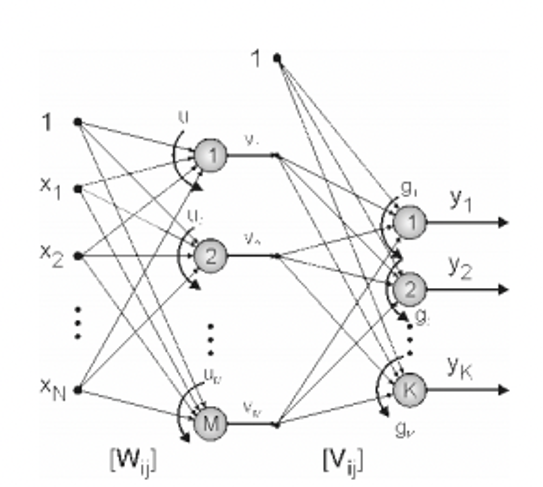
\includegraphics[scale=0.75]{./content/images/2-5.png}
    \caption{Cấu trúc mạng MLP với một tầng vào, một tầng ẩn và một tầng ra}
    \label{fig:2-5}
\end{figure}

Mạng MLP với một tầng ẩn có thể được đặc trưng bởi các thông số sau:
\begin{itemize}
\item Bộ ba (\textit{N}, \textit{M}, \textit{K}), trong đó \textit{N} − số đầu vào, \textit{M} − số nơ-ron thuộc tầng ẩn, \textit{K} − số nơ-ron ở tầng đầu ra.
\item Các hàm truyền đạt: $f_{1}$ của tầng ẩn và $f_{2}$ của tầng đầu ra.
\item Ma trận trọng số \textit{W} kết nối giữa tầng đầu vào và tầng ẩn, ma trận trọng số kết nối \textit{V} giữa tầng ẩn và tầng đầu ra.
\end{itemize}

Khi đó, với véc tơ đầu vào \textit{x} = [$x_{1}$, $x_{2}$,...,$x_{N}$] $\in$ $R^{N}$ (đầu vào phân cực cố định $x_{0}$ = 1), ta có đầu ra được xác định tuần tự theo chiều \textit{lan truyền thuận} (forward propagation) như sau:

\begin{enumerate}
\item Tính tổng các kích thích đầu vào của nơ-ron ẩn thứ \textit{i} (cho \textit{i} = 1,2,...,\textit{M}):

\begin{equation}
\label{eq:1}
u_{i} = \sum_{j=0}^{N}x_{j}W_{ij}
\tag{1}
\end{equation}

\item Tính đầu ra của nơ-ron thứ \textit{i} (cho \textit{i} = 1,2,...,\textit{M}):

\begin{equation}
\label{eq:2}
v_{i} = f_{1}(u_{i})
\tag{2}
\end{equation}

\item Tính tổng kích thích đầu vào của nơ-ron đầu ra thứ \textit{i} (cho \textit{i} = 1,2,...,\textit{M}):

\begin{equation}
\label{eq:3}
g_{i} = \sum_{j=0}^{M}v_{j}V_{ij}
\tag{3}
\end{equation}

\item Và cuối cùng ta có đầu ra thứ \textit{i} của mạng (cho \textit{i}= 1,2,…,\textit{K}) sẽ bằng:

\begin{equation}
\label{eq:4}
y_{i} = f_{2}(g_{i})
\tag{4}
\end{equation}

\end{enumerate}

Tổng hợp lại ta có hàm truyền của mạng MLP là một hàm phi tuyến cho theo công thức phụ thuộc sau:

\begin{equation}
\label{eq:5}
y_{i} = f_{2}(g_{i}) = f_{2}\left ( \sum_{j=0}^{M}v_{j}V_{ij} \right ) = f_{2}\left ( \sum_{j=0}^{M}f_{1}(u_{j})V_{ij} \right ) = f_{2}\left ( \sum_{j=0}^{M}\left [ f_{1}\left ( \sum_{k=0}^{N}x_{k}W_{jk} \right )V_{ij} \right ] \right )
\tag{5}
\end{equation}

Quá trình điều chỉnh các thông số của mạng để thích nghi với bộ số liệu được gọi là quá trình học của mạng MLP hay còn được gọi là quá trình huấn luyện mạng MLP theo một bộ mẫu cho trước. Trong khi các thông số cấu trúc như số tầng nơ-ron, các hàm truyền đạt của mỗi tầng, số nơ-ron trên mỗi tầng thường được chọn bằng thực nghiệm hoặc bằng phương pháp thử các giá trị rời rạc nhất định thì các thông số trọng số ghép nối giữa các nơ-ron có thể được điều chỉnh thích nghi bằng các thuật toán tối ưu hóa (còn gọi là thuật toán \textit{“học”}). Khi sử dụng thuật toán bước giảm cực đại, ta cũng khởi tạo các giá trị trọng số bằng các giá trị ngẫu nhiên nào đó: $[W]=[W]^{(0)}$; $[V]=[V]^{(0)}$. Sau đó ta sẽ xây dựng các công thức lặp để điều chỉnh liên tiếp các giá trị này để hàm sai số tiến tới cực trị.

\section{Mạng nơ-ron hồi quy (Recurrent Neural Network – RNN)}
\subsection{Kiến trúc và cách thức hoạt động}
Mạng nơ-ron hồi quy RNN là một loại của mạng nơ-ron nhân tạo bao gồm các đơn vị được kết nối có hướng với nhau như một chuỗi. Trong thực tế có nhiều loại dữ liệu có sự tương hỗ ràng buộc với nhau theo thứ tự thời gian, nơi mà giá trị ở phía sau chuỗi thời gian phụ thuộc vào ngữ cảnh của một vài giá trị trước đó. Ví dụ khi chúng ta xem một bộ phim, để có thể hiểu được những diễn của bộ phim, chúng ta cần phải biết được những ngữ cảnh đã xảy ra trước đó để có thể liên kết thông tin. Điều này có nghĩ là chúng ta phải ghi nhớ được những thông tin xảy ra ở những khoảng thời gian trước đó. Với các kiến trúc mạng nơ-ron nhân tạo trước đây như \textit{mạng nơ-ron tích chập} (Convolutional Neural Networks – CNN) hay ANN, tất cả dữ liệu đầu vào là độc lập với nhau. Tuy nhiên, với thiết kế của mình, RNN có thể ghi nhớ được thông tin trước đó vì dữ liệu sẽ được đưa vào mạng theo trình tự thời gian của nó. Vì vậy, RNN có thể thể hiện được mối liên hệ giữa các giá trị của dữ liệu đầu vào.

Để đạt được điều đó, RNN tạo một mạng với vòng lặp trong nó, điều này giúp nó lưu giữ các thông tin. Chúng ta có thể hình dung đây như là sao chép của cùng một mạng và nối chúng lại thành một chuỗi dài, thông tin sẽ đường truyền theo thứ tự tới các mạng ở phía sau.

Như trong hình \ref{fig:2-6}, $x_{0}$ sẽ là đầu vào đầu tiên của chuỗi dữ liệu được đưa vào mạng, từ đó RNN sẽ tính ra kết quả h0. Sau đó $h_{0}$  kết hợp với đầu vào $x_{1}$ sẽ là thông tin để tính toán cho bước tiếp theo. Tương tự, $h_{1}$ và $x_{2}$ sẽ là dữ liệu đầu vào của bước tiếp theo và quá trình sẽ được lặp như vậy cho hết chuỗi dữ liệu đầu vào. Bằng phương pháp này, RNN có thể ghi nhớ thông tin trong quá trình huấn luyện mô hình.

\begin{figure}[H]
    \centering
    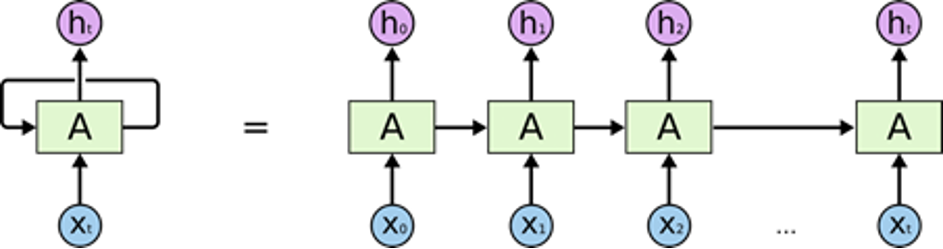
\includegraphics[scale=0.75]{./content/images/2-6.png}
    \caption{Cấu trúc mạng RNN}
    \label{fig:2-6}
\end{figure}

\subsection{Vấn đề của RNN}
Ý tưởng của RNN là liên kết thông tin trước đó để biểu diễn giá trị hiện tại, ví dụ như ngữ cảnh của từ ngữ trước đó trong câu để hiểu nghĩa của từ ngữ hiện tại. Nhưng RNN không phải lúc nào cũng có thể ghi nhớ được toàn bộ thông tin.

Nếu chúng ta đang có gắng dự đoán từ cuối trong câu \textit{"mặt trời mọc hướng đông"}, chúng ta sẽ không cần sử dụng nhiều ngữ cảnh của từ ngữ ở trước đó. Lúc này khoảng cách giữa ngữ cảnh và từ chúng ta cần dự đoán là không lớn, RNN có thể ghi nhớ được ngữ cảnh này. Tuy nhiên, xét câu sau \textit{"Tôi là công dân Việt Nam. Đó là đất nước tuyệt vời... Đất nước này thuộc châu Á"}. Rõ để có thể dự đoán được từ cuối cùng trong câu là \textit{châu Á}, chúng ta cần phải nhớ được thông tin \textit{Việt Nam} đã được nhắc đến từ lâu ở trước đó. Lúc này, khoảng cách giữa ngữ cảnh cần liên kết với từ cần dự đoán lớn, vì vậy RNN sẽ không thể lưu giữ thông tin của ngữ cảnh vì sau một chuỗi truyền thông tin dài qua các mạng, những thông tin ở xa trước đó sẽ bị triệt tiêu. Điều này đã được Bengio và các cộng sự tìm ra và lý giải \cite{st18}.

\section{Mạng nơ-ron học sâu Long Short-Term Memory (LSTM)}
Mạng nơ-ron học sâu LSTM, là một dạng đặc biệt của RNN, có khả năng học được những sự phụ thuộc trong một thời gian dài, được phát minh bởi Hochreiter và Schmidhuber \cite{st11}. LSTM được thiết kế để giải quyết vấn đề triệu tiêu thông tin của RNN. Tất cả mạng RNN có dạng của một chuỗi lặp lại của các khối mạng nơ-ron. Các khối này có cấu trúc khá đơn giản, như chỉ là một hàm kích hoạt \textit{tanh} như hình \ref{fig:2-7}.

\begin{figure}[H]
    \centering
    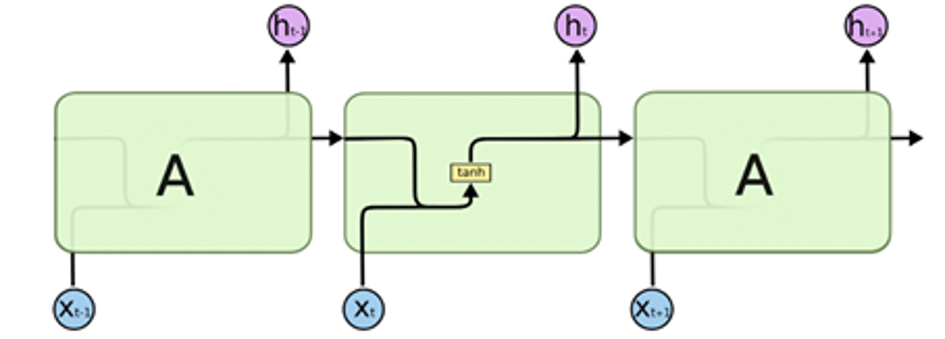
\includegraphics[scale=0.75]{./content/images/2-7.png}
    \caption{Sự lặp lại của các khối nơ-ron trong kiến trúc RNN tiêu chuẩn}
    \label{fig:2-7}
\end{figure}

\begin{figure}[H]
    \centering
    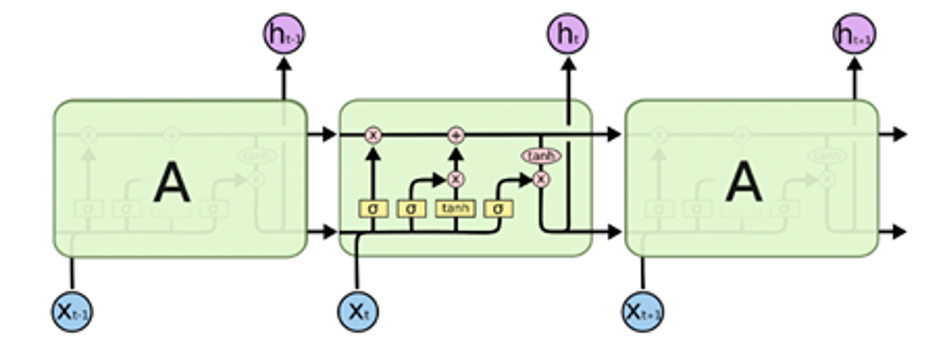
\includegraphics[scale=0.75]{./content/images/2-8.png}
    \caption{Sự lặp lại của các khối nơ-ron trong kiến trúc LSTM}
    \label{fig:2-8}
\end{figure}

LSTM cũng kế thừa chuỗi lặp lại các khối nơ-ron như RNN, nhưng các khối này khác cấu trúc so với bản tiêu chuẩn như hình \ref{fig:2-8}. Thay vì chỉ đơn thuần là một tầng nơ-ron đơn giản, khối này gồm bốn hàm (function) với các chức năng riêng biệt của mình. Hình \ref{fig:2-9} mô tả kiến trúc của một đơn vị LSTM.

\begin{figure}[H]
    \centering
    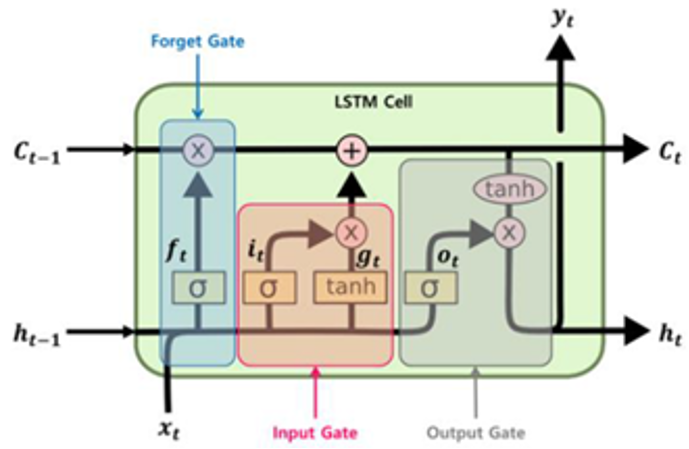
\includegraphics[scale=0.75]{./content/images/2-9.png}
    \caption{Kiến trúc một đơn vị LSTM}
    \label{fig:2-9}
\end{figure}

\textbf{Forget Gate: } Chịu trách nhiệm xóa bỏ những thông tin không cần thiết từ đơn vị LSTM phía trước. Trong phương trình (\ref{eq:6}), $f_t$ là đầu ra của Forget Gate tại thời điểm hiện tại,  $\sigma$ là ký hiệu của hàm \textit{sigmoid}, $C_{t-1}$ và $h_{t-1}$ tuần tự là trạng thái của đơn vị LSTM (cell state) và đầu ra của tầng ẩn tại thời điểm trước đó. $W_f$ và $b_f$ tuần tự là độ dài vec-tơ và bias từ tầng đầu vào cho tới Forget Gate.

\begin{equation}
\label{eq:6}
f_t = \sigma(W_f[C_{t-1},h_{t-1},x_t] + b_f)
\tag{6}
\end{equation}

\textbf{Input Gate: } Lựa chọn những thông tin cần thiết để thêm vào trạng thái của đơn vị
LSTM. Input Gate bao gồm 02 phần: tầng \textit{sigmoid} and tầng \textit{tanh}. tầng \textit{sigmoid} lọc thông tin từ $h_{t-1}$ và $C_{t-1}$. tầng \textit{tanh} tạo các giá trị thích hợp sẽ được thêm vào bộ nhớ LSTM. Đầu ra của 02 tầng này được tính toán bởi các công thức sau:

\begin{equation}
\label{eq:7}
i_t = \sigma(W_i[C_{t-1},h_{t-1},x_t] + b_i)
\tag{7}
\end{equation}
\begin{equation}
\label{eq:8}
\c{C}_t = \textit{tanh}(W_c[h_{t-1},x_t] + b_c)
\tag{8}
\end{equation}

Trong phương trình  (\ref{eq:7}), $i_t$ là đầu ra của Input Gate. $W_i$ và $b_i$ là độ dài vectơ và bias của Input Gate. $W_c$ và $b_c$ trong phương trình (\ref{eq:8})là độ dài vec-tơ và bias của trạng thái đơn vị LSTM.

Trạng thái đơn vị LSTM phía trước $C_{t-1}$ được cập nhật cho $C_t$ bằng phép nhân trạng thái đơn vị LSTM phía trước và sau đó cộng thêm $i_t$ * $\c{C}_t$ , thông tin mới được quyết
định để nhớ. Bước này được mô tả trong phương trình (\ref{eq:9}).

\begin{equation}
\label{eq:9}
C_t = f_t * C_{t-1} + i_t * \c{C}_t
\tag{9}
\end{equation}

\textbf{Output Gate: } Xác định thông tin từ trạng thái đơn vị LSTM được sử dụng làm đầu ra. Trong phương trình (\ref{eq:10}) và (\ref{eq:11}), $o_t$ là đầu ra của Output Gate, $W_0$ và $b_0$ là độ dài vec-tơ và \textit{bias} từ Input Gate đến Output gate, và $h_t$ là đầu ra của tầng ẩn tại thời điểm hiện tại.

\begin{equation}
\label{eq:10}
o_t = \sigma(W_o[C_{t},h_{t-1},x_t] + b_o)
\tag{10}
\end{equation}
\begin{equation}
\label{eq:11}
h_t = o_t * tanh(C_t)
\tag{11}
\end{equation}

Điểm chính của mạng nơ-ron học sâu LSTM được gọi là \textit{trạng thái khối} (cell state). Nó có khả năng thêm hoặc xóa bớt thông tin của trạng thái khối thông qua các cổng. \textit{Cổng} (Gate) là cách để tùy chỉnh lượng thông tin được truyền trải qua.

Nó kết hợp với hàm kích hoạt \textit{sigmoid}, giá trị nằm giữa 0 và 1, sẽ biểu thị bao nhiêu thông tin được truyền tải qua. Khi sigmoid có giá trị 0 có nghĩa là không có chút thông tin nào được đi qua, trong khi gía trị 1 có nghĩa là tất cả thông tin được phép truyền đi tiếp. LSTM có tổng cộng 3 \textit{cổng}, để điều khiển và bảo vệ \textit{trạng thái khối}.

\section{Mạng nơ-ron học sâu LSTM xếp chồng (Stacked LSTM Network)}
Mạng nơ-ron học sâu LSTM truyền thống bao gồm một tầng LSTM ẩn duy nhất, theo sau đó là tầng xuất truyền thẳng tiêu chuẩn. \textit{Mạng nơ-ron học sâu LSTM xếp chồng} (Stacked LSTM Network) là một phần mở rộng của loại mô hình này, trong đó có nhiều tầng LSTM ẩn, mỗi tầng LSTM ẩn chứa nhiều đơn vị (như trong hình \ref{fig:2-10}). Việc xếp chồng này sẽ làm cho mạng sâu hơn, ước lượng tốt hơn những hàm phi tuyến, tăng độ chính xác. Độ sâu của mạng nơ-ron được cho là đóng góp vào sự thành công của mạng nơ-ron học sâu \cite{st19}.

\begin{figure}[ht]
    \centering
    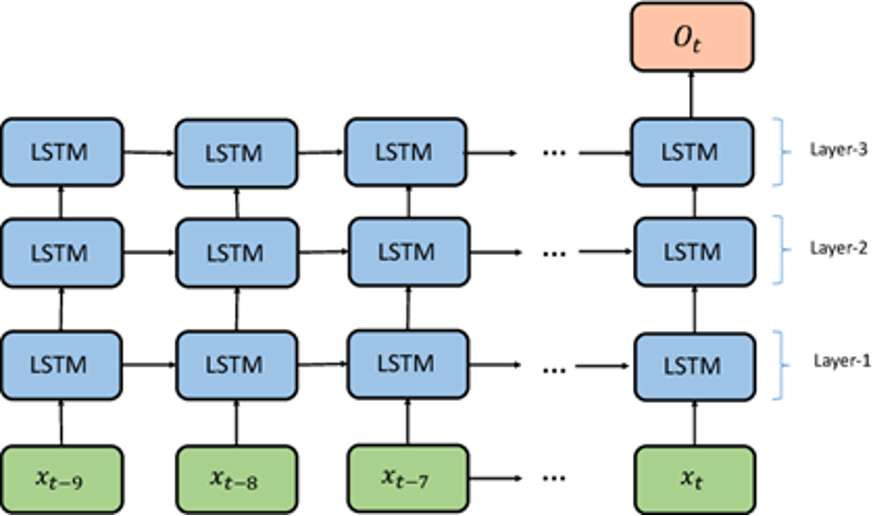
\includegraphics[scale=0.7]{./content/images/2-10.png}
    \caption{Kiến trúc LSTM xếp chồng}
    \label{fig:2-10}
\end{figure}

Các tầng ẩn bổ sung có thể được thêm vào để làm cho mạng sâu hơn. Các tầng ẩn được thêm vào có thể được hiểu là kết hợp lại các biểu diễn đã học từ các tầng trước và tạo ra các biểu diễn mới ở mức trừu tượng cao hơn. Ví dụ, từ đường nét đến hình dạng
của đối tượng.

Một tầng ẩn đủ lớn cũng có thể xấp xỉ bất kỳ hàm phi tuyến nào. Nhưng việc tăng độ sâu của mạng sẽ làm cho số nơ-ron mỗi tầng ít lại và thời gian huấn luyện cũng được giảm bớt \cite{st20}. Điều này cũng được áp dụng cho mạng nơ-ron học sâu LSTM xếp chồng. Ngoài ra, mạng nơ-ron học sâu LSTM hoạt động trên dữ liệu chuỗi thời gian, điều này
có nghĩa là việc thêm vào các tầng ẩn sẽ làm tăng mức trừu tượng của các quan sát đầu vào theo thời gian. Mạng LSTM xếp chồng được nghiên cứu bởi Graves và các cộng sự \cite{st21}. Theo nghiên cứu này, hiệu quả vượt trội so với các công trình đi trước. Graves và các cộng sự cũng tìm ra rằng độ sâu của mạng quan trọng hơn số nơ-ron trong mỗi tầng ẩn.

\vspace{0.5cm}

\begin{figure}[H]
    \centering
    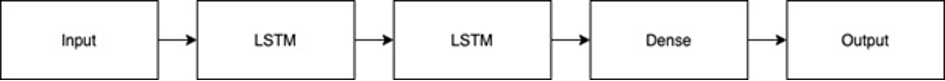
\includegraphics[scale=0.75]{./content/images/2-11.png}
    \caption{Mạng LSTM xếp chồng}
    \label{fig:2-11}
\end{figure}


Kiến trúc LSTM xếp chồng có thể được định nghĩa như một mô hình LSTM bao gồm nhiều tầng LSTM. Một tầng LSTM ở trước cung cấp một đầu ra, và nó được sử dụng làm đầu vào cho tầng LSTM ở sau (như trong hình \ref{fig:2-11}). Mạng LSTM xếp chồng hiện là một kỹ thuật ổn định và hiệu quả cho các bài toán dự đoán dữ liệu có trình tự.